\documentclass[svgnames]{beamer}

\usetheme{Dresden}
\usecolortheme{beaver}

\usepackage{import, fancybox, graphicx, color, colortbl, bm}

\newcommand{\ssline}{\vspace{8 pt}}

\title{TCP ex Machina: \\Computer-Generated Congestion Control}

\author{Keith~Winstein and Hari~Balakrishnan}
\institute{MIT Computer Science and Artificial Intelligence Laboratory\\\vspace{\baselineskip}\textcolor{DarkBlue}{http://web.mit.edu/remy}}
\date{August 14, 2013}

\begin{document}

\begin{frame}[plain]

\titlepage

\end{frame}

\institute{MIT Computer Science and Artificial Intelligence Laboratory}

\section{Introduction}

\begin{frame}
\frametitle{Congestion control!}

\begin{itemize}

\Large

\item Prevents congestion collapse

\item Allocates network resources among users

\item Can be purely end-to-end or not

\end{itemize}

\end{frame}

\begin{frame}
\frametitle{The march of congestion control mechanisms}
\only<1>{\noindent \hspace{-.75 cm} 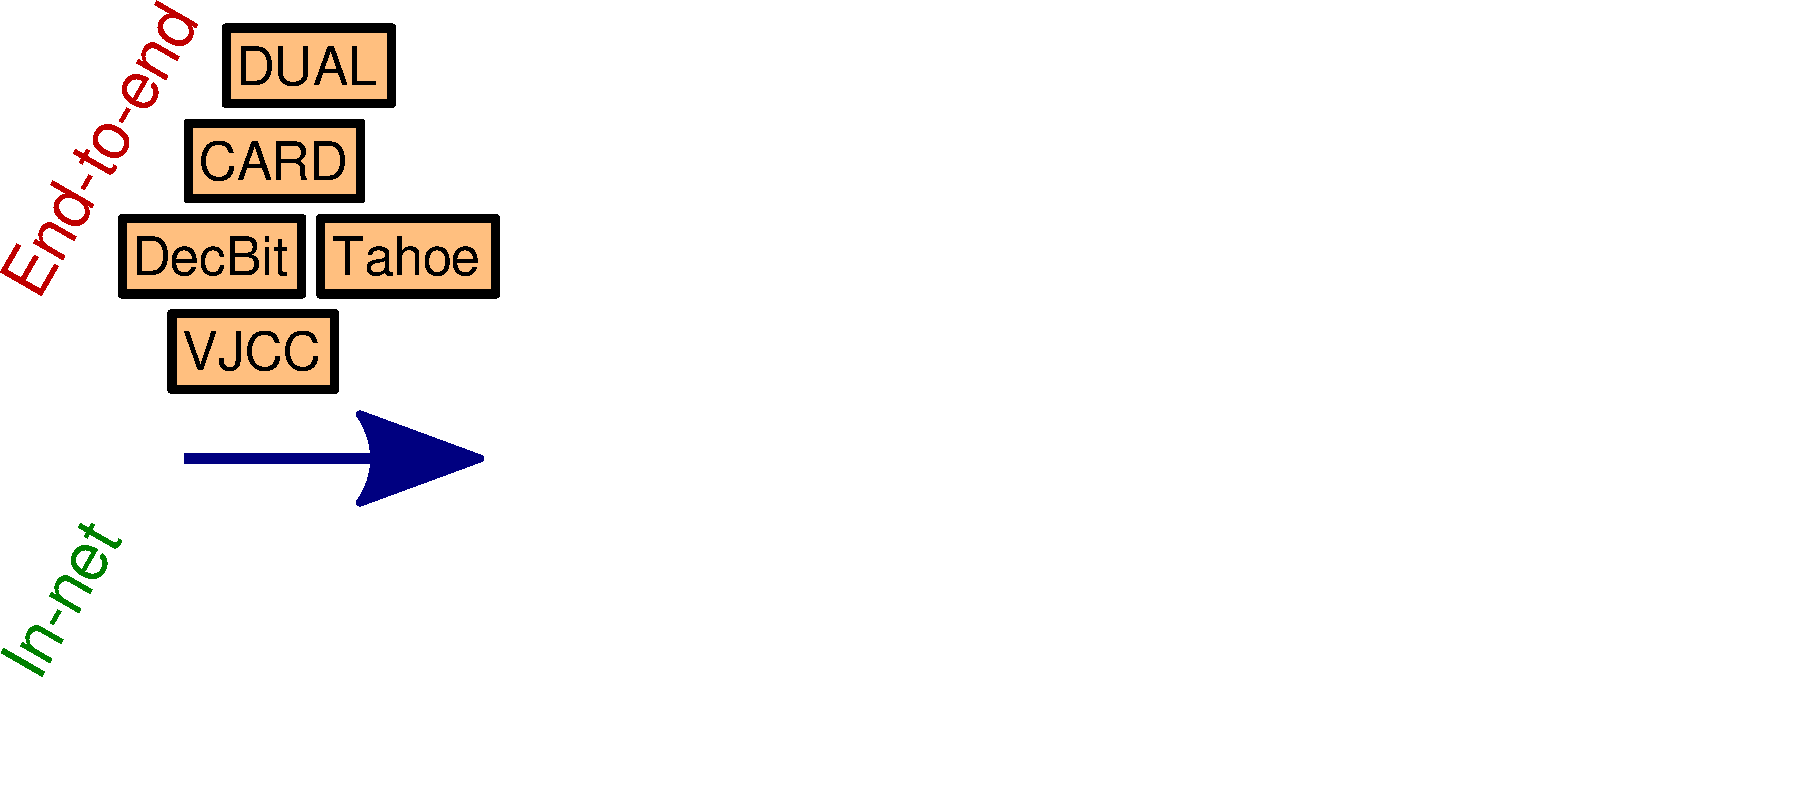
\includegraphics[width=1.1\textwidth]{march-4.pdf}

}
\only<2>{\noindent \hspace{-.75 cm} 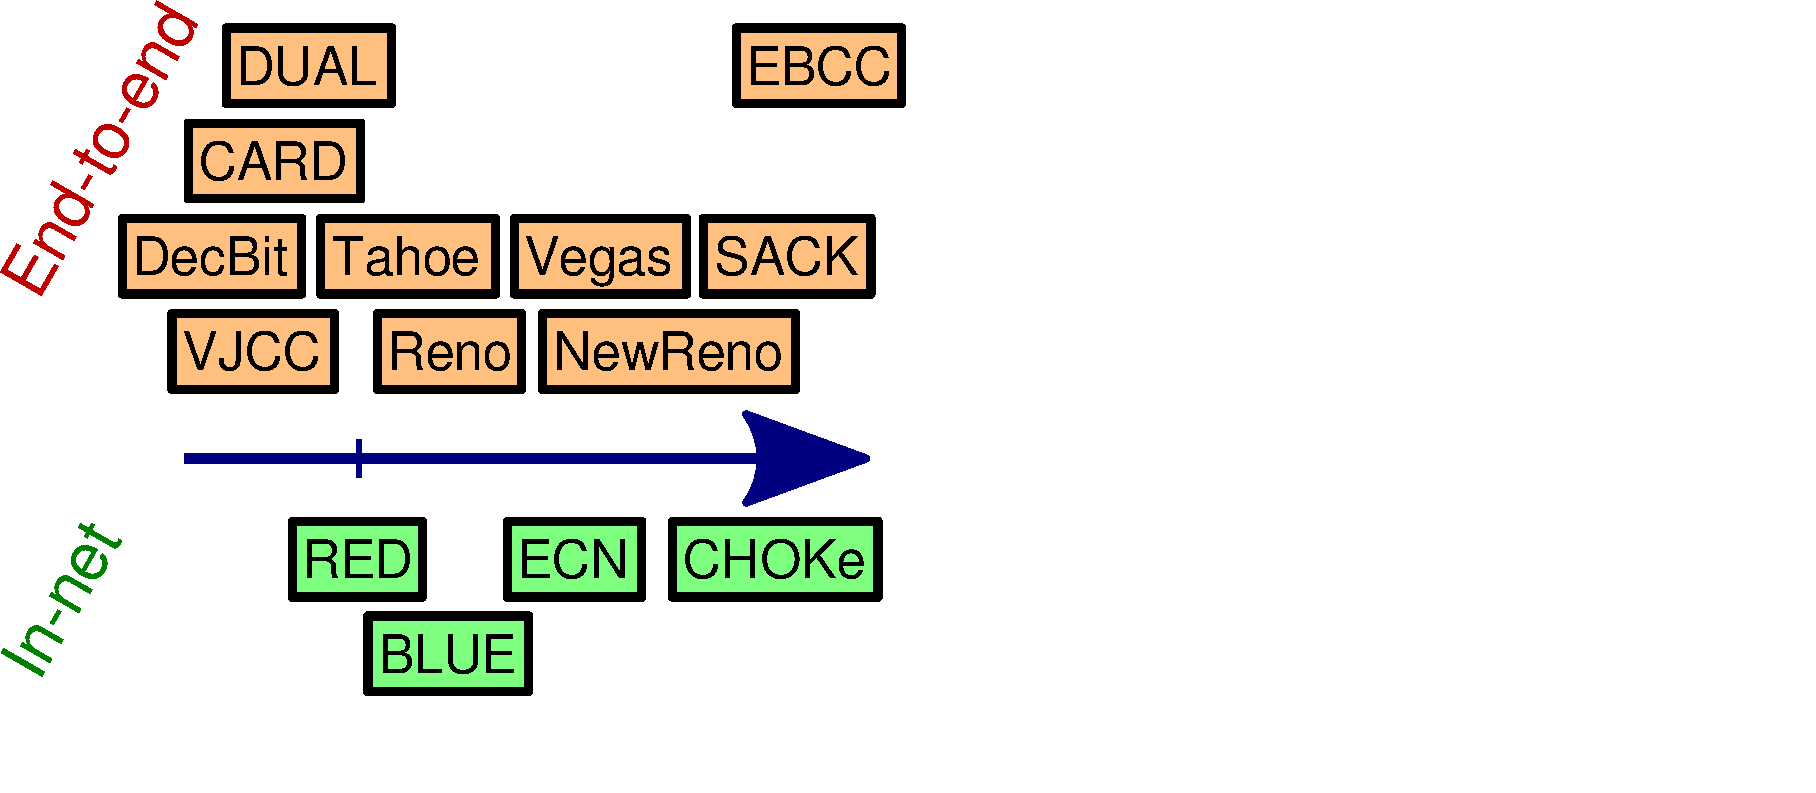
\includegraphics[width=1.1\textwidth]{march-3.pdf}

}
\only<3>{\noindent \hspace{-.75 cm} 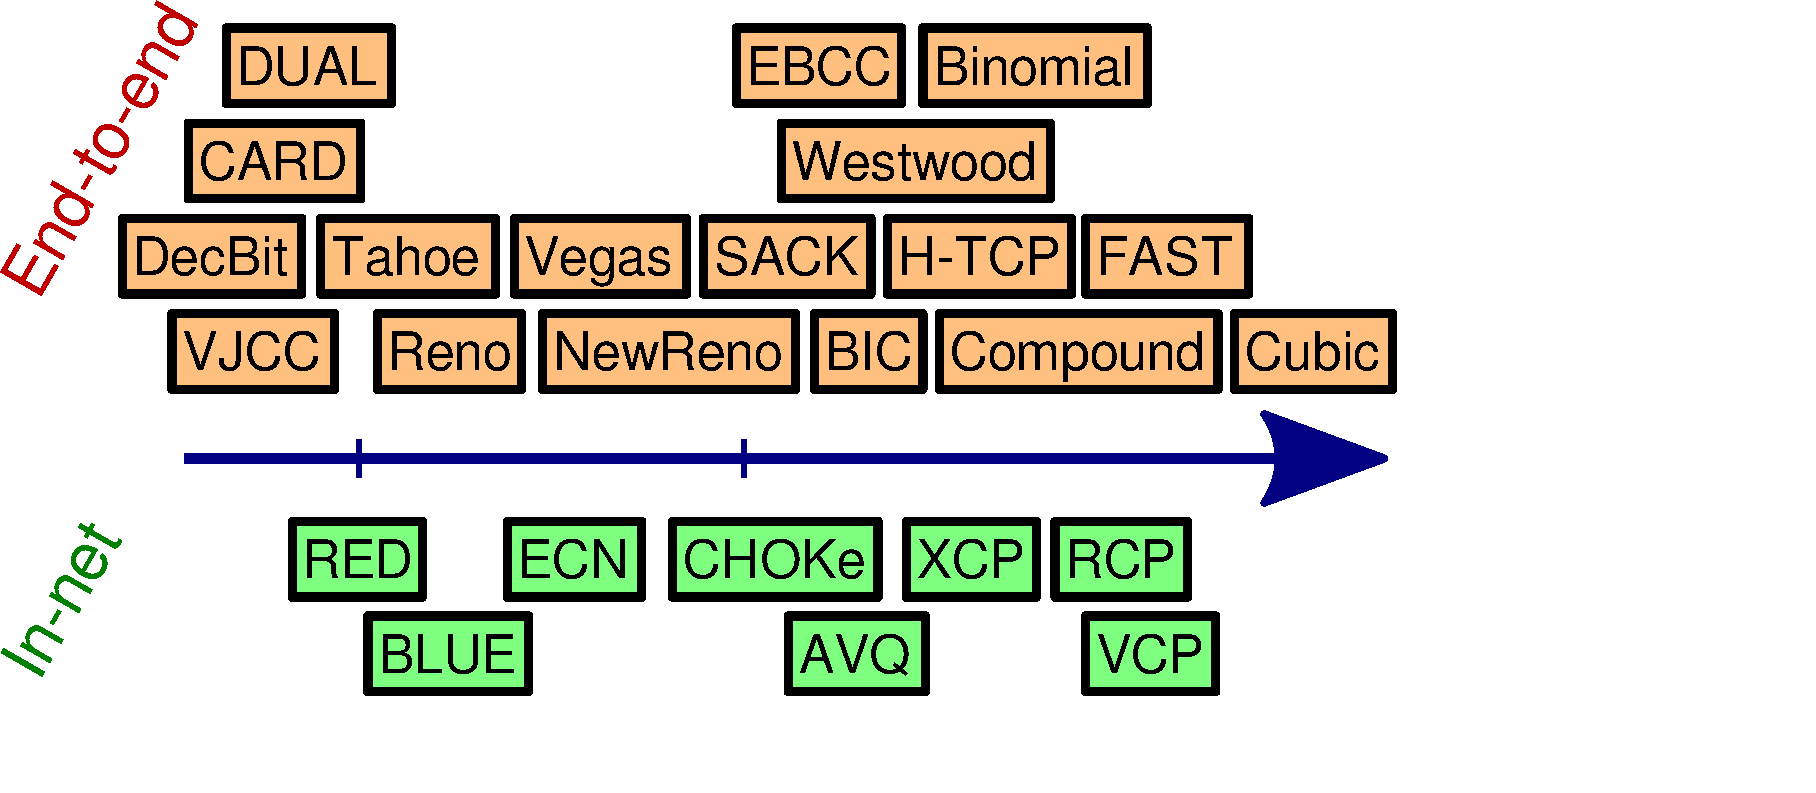
\includegraphics[width=1.1\textwidth]{march-2.pdf}

}
\only<4>{\noindent \hspace{-.75 cm} 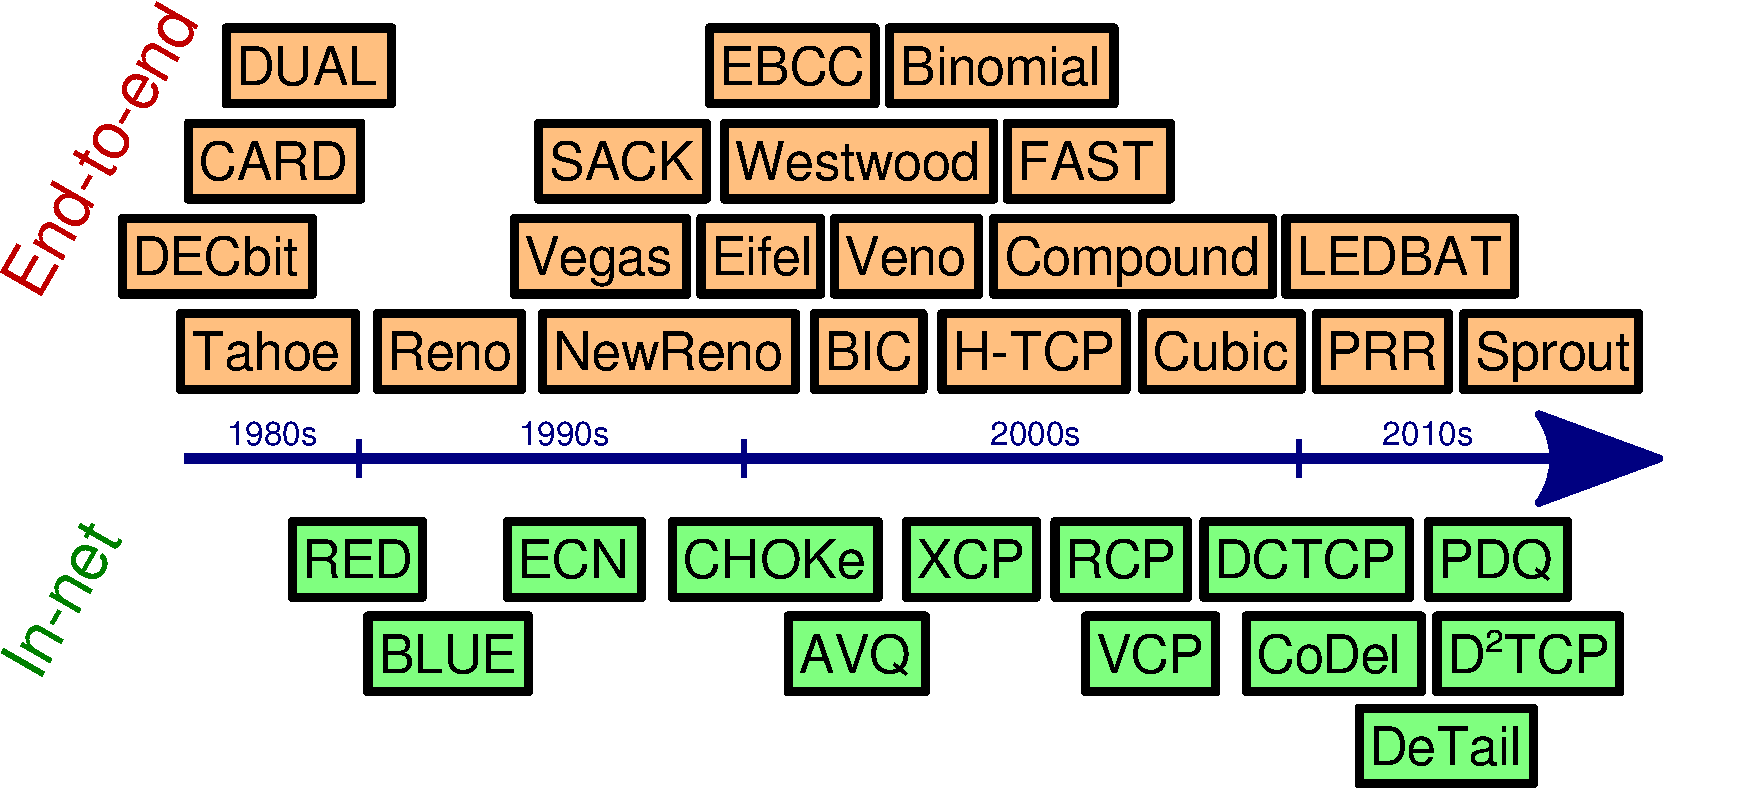
\includegraphics[width=1.1\textwidth]{march-1.pdf}

}
\only<5>{\noindent \hspace{-.75 cm} 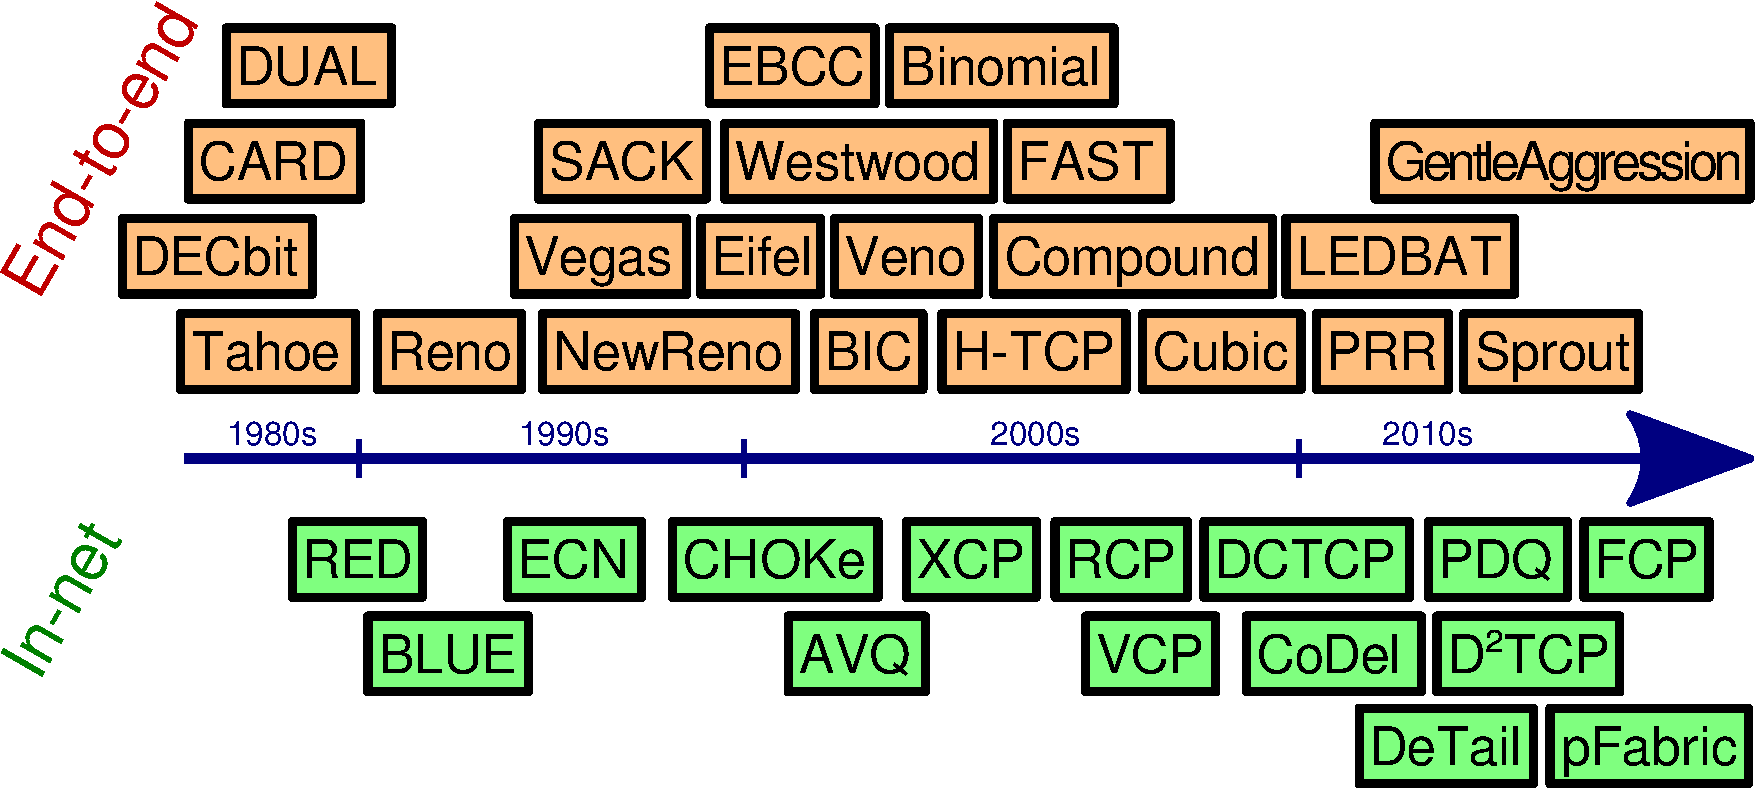
\includegraphics[width=1.1\textwidth]{march.pdf}

}
\end{frame}

%\begin{frame}
%\begin{centering}
%\LARGE One size does not fit all.
%
%\end{centering}
%\end{frame}

\begin{frame}

\frametitle{Our work}

\begin{centering}

\LARGE \textcolor{DarkGreen}{If congestion control is the answer,\\what's the question?}

\vspace{\baselineskip}

\pause

\LARGE \textcolor{NavyBlue}{Are there better answers?}

\end{centering}

\end{frame}

\begin{frame}
\frametitle{Rational choice of scheme is challenging}

\begin{centering}

\includegraphics[height=20 pt]{cubic.pdf}\hspace{8 pt}{\bf vs.}\hspace{8 pt}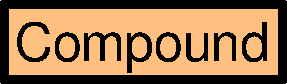
\includegraphics[height=20 pt]{compound.pdf}

\end{centering}

\ssline
\ssline
\ssline

\begin{itemize}

\Large

\item Different goals?

\item Different assumptions about network?

\item One scheme just plain better?

\end{itemize}

\end{frame}

\begin{frame}
\frametitle{What are the ends that TCP tries to achieve?}

\begin{itemize}

\Large

\item ``Teleology of TCP'' is mostly unknown

\item Asymptotic solutions for long-running flows

\item Dynamical behavior is complex

\end{itemize}

\end{frame}

\begin{frame}
\frametitle{Networks constrained by a fuzzy idea of TCP's assumptions}

\Large

\begin{itemize}
\item Mask stochastic loss
\item Bufferbloat
\item Mask out-of-order delivery
\item No parallel/multipath routing
\item[]
\item[] {\it Advice for Internet Subnetwork Designers}\\ (RFC 3819, July 2004) is 21,000 words!
\end{itemize}

\end{frame}

\begin{frame}
\frametitle{Apps hack around TCP}

\Large

\begin{itemize}
\item Open lots of flows \hspace{1.9 cm} \only<2->{
\includegraphics[width=0.5cm]{firefox.png} \hspace{0.001 cm} 
\includegraphics[width=0.5cm]{chrome-64.png} \hspace{0.001 cm} 
\includegraphics[width=0.5cm]{Internet_Explorer_10_logo.png} \hspace{0.02 cm} 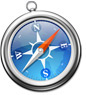
\includegraphics[width=0.5cm]{safari.jpg} \hspace{0.02 cm} 
\includegraphics[width=0.5cm]{mozilladino.png}}

\item Goose slow start \only<3->{\hspace{2.18 cm} \raisebox{-0.6ex}{
\includegraphics[height=14 pt]{Google_Logo_Old.PNG}} \raisebox{-.125 ex}{
\includegraphics[height=10 pt]{mslogo.png}}}

\item Add pacing \hspace{3.3 cm} \only<4->{\raisebox{-.4 ex}{
\includegraphics[height=14 pt]{youtube.png}}}

\item Give up and do it yourself

\visible<5>{
\small
\hspace{5.95 cm}\begin{minipage}{3.5 cm}
{\bf Chrome} \textcolor{DarkBlue}{(QUIC)} \\
{\bf BitTorrent} \textcolor{DarkBlue}{($\mu$TP)} \\
{\bf Mosh} \textcolor{DarkBlue}{(SSP)} \\
{\bf Aspera} \textcolor{DarkBlue}{(fasp)} \\
\end{minipage}
}

\end{itemize}

\end{frame}

\begin{frame}
\frametitle{Better: free the network to evolve}

\Large Transport layer should adapt to \textbf{\textcolor{DarkBlue}{whatever}}:

\begin{itemize}
\item network does

\item application wants

\end{itemize}

\end{frame}

\begin{frame}
\frametitle{What we built}

\colorbox{Bisque}{
\begin{centering}
\noindent \begin{tabular}{ll}
\Large \textcolor{DarkRed}{\bf Remy}: & \Large a program that generates \\ & \Large congestion-control schemes offline
\end{tabular}

\end{centering}}

\ssline
\ssline

\textcolor{DarkBlue}{\bf Input:}

\begin{itemize}
\item Prior assumptions \hspace{3.01 cm} \textcolor{DarkBlue}{(what network may do)}

\item Goal \hspace{5.275 cm}\textcolor{DarkBlue}{(what app wants)}
\end{itemize}

\textcolor{DarkBlue}{\bf Output:} CC algorithm for a TCP sender \hspace{0.177 cm}\textcolor{DarkBlue}{(RemyCC)}

\ssline

\textcolor{DarkBlue}{\bf Time:} a few hours

\ssline

\textcolor{DarkBlue}{\bf Cost:} \$5--\$10 on Amazon EC$^2$

\end{frame}

\begin{frame}
\frametitle{The basic question of congestion control}

\section{The problem}

\begin{centering}
\fbox{
\begin{minipage}{6 cm}
\LARGE At this moment, do I:

\begin{itemize}

\item send a packet
\item not send a packet?

\end{itemize}

\end{minipage}
}

\end{centering}

\end{frame}

\begin{frame}
\frametitle{Dumbbell network}

\only<1>{\noindent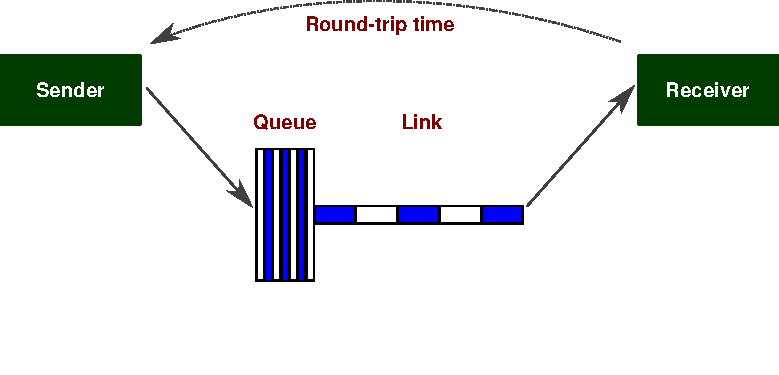
\includegraphics[width=\textwidth]{dumbbell-2.pdf}}\only<2>{\noindent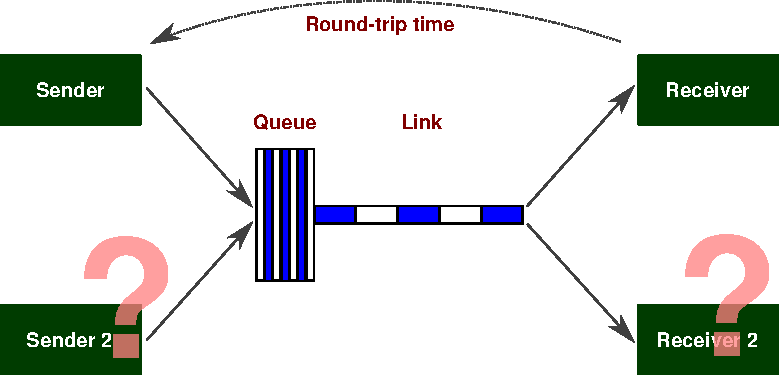
\includegraphics[width=\textwidth]{dumbbell-1.pdf}}\only<3>{\noindent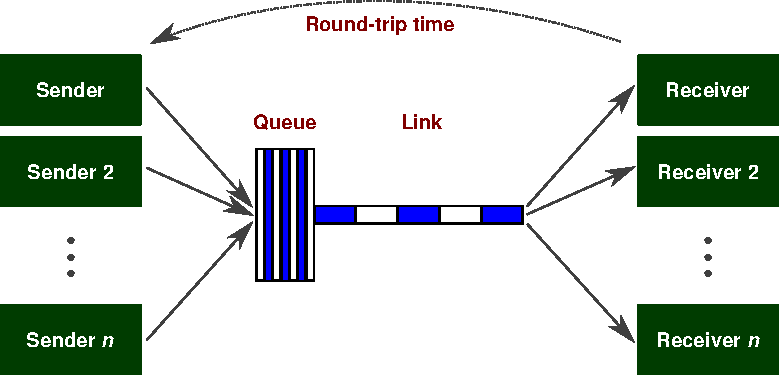
\includegraphics[width=\textwidth]{dumbbell.pdf}}

\end{frame}

%\begin{frame}
%\frametitle{The goal}
%
%\Large
%
%\begin{itemize}
%
%\item Tradeoff between \textbf{efficiency} and \textbf{fairness}
%
%\item Tradeoff between \textbf{throughput} and \textbf{delay}
%
%\end{itemize}
%
%\end{frame}

\begin{frame}
\frametitle{Objectives of congestion control}

\textbf{Minimize}

\begin{itemize}
\item average flow completion time

\item page load time

\item tail completion time

\end{itemize}

\textbf{Maximize}

\begin{itemize}

\item \begin{minipage}{3.75 cm}
$\min_i \textsf{throughput}_i$
\end{minipage} \textsf{\textcolor{DarkBlue}{(max-min throughput)}}

\item \begin{minipage}{3.75 cm}
\[\sum_i \log \left[ \textsf{throughput}_i \right]\]
\end{minipage} \textsf{\textcolor{DarkBlue}{(proportionally fair throughput)}}

\item
\begin{minipage}{3.75 cm}
\begin{tabular}{l}
\cellcolor{Bisque}\raisebox{0.75 cm}{\begin{minipage}{3.75 cm}
\[\sum_i \log \left[ \frac{\textsf{throughput}_i}{\visible<2>{
\textcolor{DarkBlue}{\big(}
}\textsf{delay}_i\visible<2>{
\textcolor{DarkBlue}{\big)^{\bm \delta}}}} \right]\]
\end{minipage} \textsf{\textcolor{DarkBlue}{(proportionally fair throughput/delay)}}}
\end{tabular}
\end{minipage}

\end{itemize}

\end{frame}

\begin{frame}
\frametitle{Prior knowledge}

\begin{itemize}

\Large

\item Model of network uncertainty

\begin{itemize}
\item Link speed distribution
\item Delay distribution
\end{itemize}

\item Traffic model

\begin{itemize}
\item Web browsing, MapReduce, videoconferencing
\end{itemize}

\item May be \textcolor{Red}{specific} or \textcolor{DarkBlue}{not very informative} \\

\vspace{4 pt}

\tiny \hspace{1.6 cm} \textcolor{Red}{(E.g., XCP, pFabric)} \hspace{0.2 cm} \textcolor{DarkBlue}{(Tahoe, Reno, Cubic)}
\end{itemize}

\end{frame}

\begin{frame}
\frametitle{Statement of the problem}

\Large

\begin{itemize}

\item Endpoints have no control over routing

\item Each sender only gets own receiver's acks

\item Goal: \textbf{\textcolor{DarkBlue}{optimize expected value of objective}}

%\item[] \normalsize $\Rightarrow$ decentralized partially-observable Markov decision process

\end{itemize}

\end{frame}

\begin{frame}
\frametitle{The intractable question of congestion control}

\begin{centering}
\fbox{
\begin{minipage}{6 cm}
\LARGE At this moment,\textcolor{DarkBlue}{\bf *} do I:

\begin{itemize}

\item send a packet
\item not send a packet?

\end{itemize}

\end{minipage}
}

\ssline
\ssline
\ssline

\pause

\end{centering}

\Large \noindent \hspace{-.5cm} \mbox{\textcolor{DarkBlue}{\textbf{*} Given {\bf full history} of packets sent and acks received!}}

\end{frame}

\begin{frame}
\frametitle{Remy: tractable search for the best}

\section{Remy}

\large

\begin{itemize}

\item Remy searches for the best congestion-control algorithm

\begin{itemize}
\item optimizes given objective over prior assumptions about network
\end{itemize}

\item \textbf{\textcolor{DarkBlue}{Approximates}} solution by limiting available state

\end{itemize}

\end{frame}

\begin{frame}
\frametitle{A RemyCC tracks three congestion signals}

\Large

\noindent \hspace{-0.75 cm}\begin{tabular}{ll}
\textcolor{DarkBlue}{$r\_ewma$}: & moving average of interval between acks \\

\textcolor{DarkBlue}{$s\_ewma$}: & \ldots between sender timestamps echoed in acks \\

\textcolor{DarkBlue}{$rtt\_ratio$}: & ratio of last RTT to smallest RTT so far \\

\end{tabular}

\end{frame}

\begin{frame}
\frametitle{Why these three congestion signals?}

\Large

\begin{itemize}

\item Benefit can be measured empirically

\begin{itemize}
\item In our experiments, little help from adding more
\item Other networks might find differently
\end{itemize}

\item More signals increase search time

\end{itemize}

\end{frame}

\begin{frame}
\frametitle{A RemyCC maps each state to an action}

\Large

\[\textsc{Rule}( \textcolor{DarkBlue}{r\_ewma}, \textcolor{DarkBlue}{s\_ewma}, \textcolor{DarkBlue}{rtt\_ratio} ) \rightarrow \langle \textcolor{Red}{m}, \textcolor{Red}{b}, \textcolor{Red}{r} \rangle \]

\ssline
\ssline

\begin{tabular}{ll}

\textcolor{Red}{$m$} & Multiple to congestion window \\

\textcolor{Red}{$b$} & Increment to congestion window \\

\textcolor{Red}{$r$} & Minimum interval between two outgoing packets \\

\end{tabular}

\end{frame}

\begin{frame}
\frametitle{Runtime for a RemyCC}

\large

\textbf{On ack:}

\begin{itemize}
\item $\langle \textcolor{Red}{m}, \textcolor{Red}{b}, \textcolor{Red}{r}\rangle \leftarrow \textsc{Rule}( \textcolor{DarkBlue}{r\_ewma}, \textcolor{DarkBlue}{s\_ewma}, \textcolor{DarkBlue}{rtt\_ratio} )$

\item $\texttt{cwnd} \leftarrow \textcolor{Red}{m} \cdot \texttt{cwnd} + \textcolor{Red}{b}$
\end{itemize}

\textbf{Send packet if:}

\begin{itemize}
\item $\texttt{cwnd} > \texttt{FlightSize}$, and

\item last packet sent $> \textcolor{Red}{r}$ ago
\end{itemize}

\end{frame}

\begin{frame}
\frametitle{Remy's job}

\Large

\colorbox{Bisque}{
\begin{minipage}{\textwidth}
Find piecewise-continuous \textsc{Rule}() that optimizes \\ expected value of objective function.

\end{minipage}}

\end{frame}

\begin{frame}
\frametitle{The algorithm (illustration TKTKTKTK)}

\begin{itemize}
\item Initially: one default rule for whole state space

\item Find best action for whole state space

\item Subdivide rule at median query $\rightarrow$ 8 new rules

\item Repeat

\end{itemize}

\ssline

Optimize existing rules and rule structure \textbf{in parallel}.

\end{frame}

\begin{frame}
\frametitle{Fixed 15 Mbps link, 8 senders, flows exp-distributed}

\section{Experiments}

\noindent 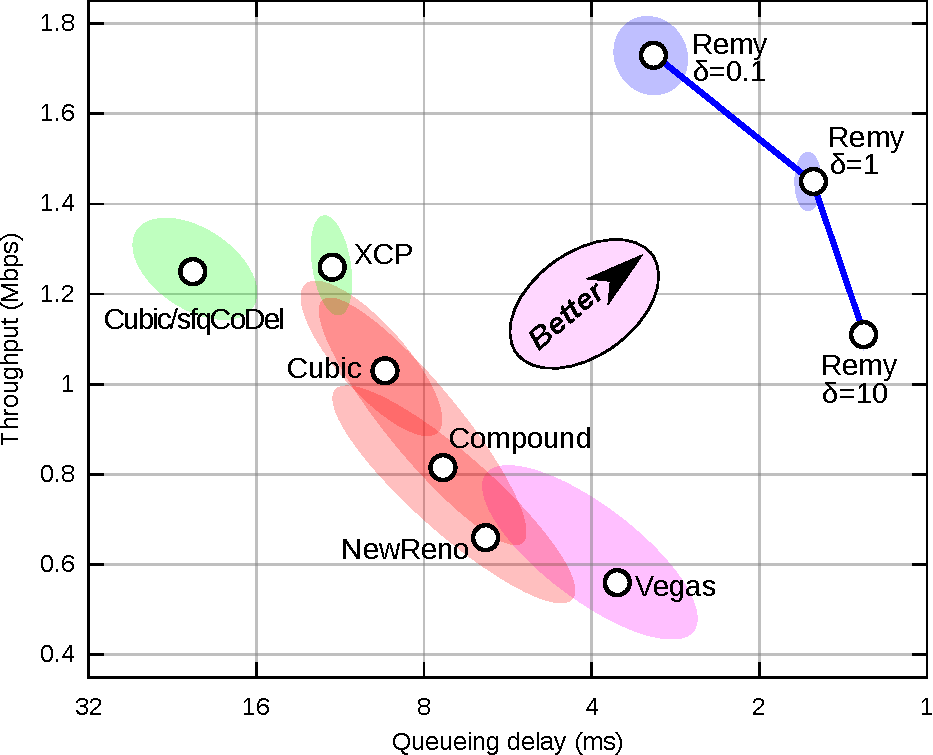
\includegraphics[width=8.5 cm]{eth8-final-bytes.pdf}

\end{frame}

\begin{frame}

\noindent 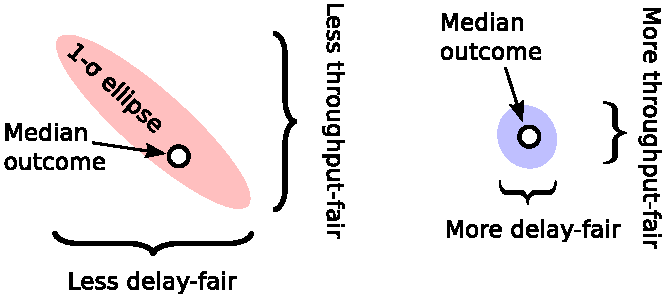
\includegraphics[width=8.5 cm]{legend.pdf}

\end{frame}

\begin{frame}
\frametitle{Fixed 15 Mbps link, 12 senders, heavy-tailed flows}

\noindent 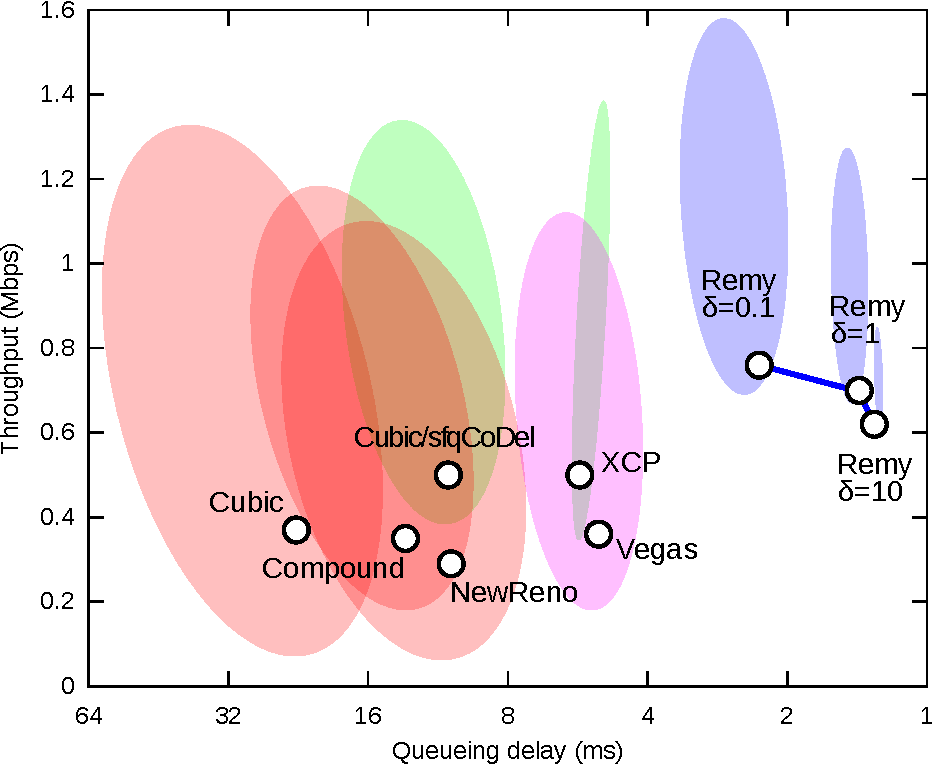
\includegraphics[width=8.5 cm]{eth12-final-flowcdf.pdf}

\end{frame}

\begin{frame}
\frametitle{Verizon LTE, 8 senders, flows exp-distributed}

\noindent 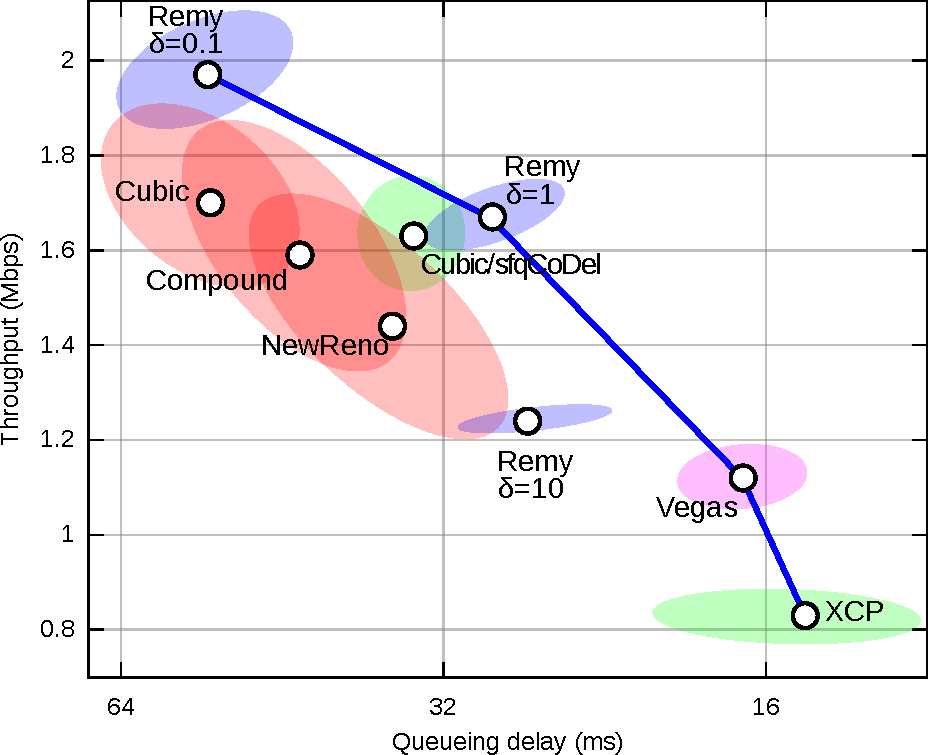
\includegraphics[width=8.5 cm]{vzw-8-final.pdf}

\end{frame}

\begin{frame}
\frametitle{Prior knowledge is helpful, when correct}

\noindent 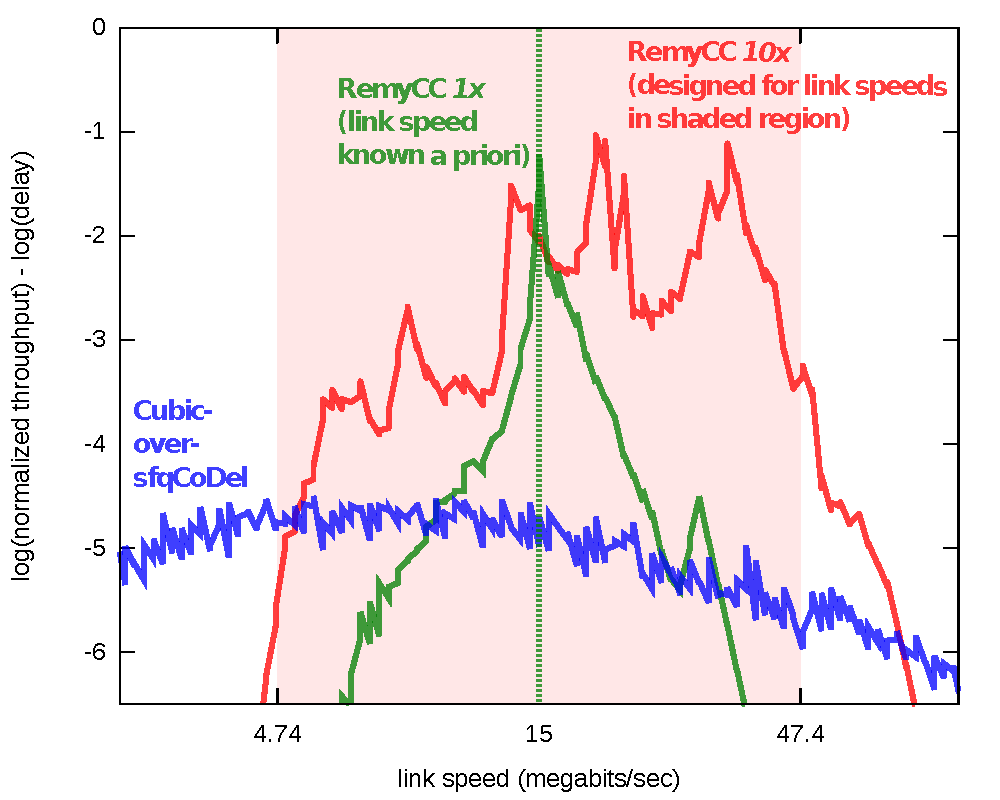
\includegraphics[width=8.5 cm]{spec2.pdf}

\end{frame}

\begin{frame}
\frametitle{Why does Remy work? TKTKTKTKTK}

\section{Discussion}

\begin{itemize}
\item Not entirely clear! (TKTKTKTK)

\item Need to reverse-engineer algorithms.

\item Hundreds of rules --- are they all necessary?
\end{itemize}

\end{frame}

\begin{frame}
\frametitle{Goal-driven algorithm \textbf{moves} the complexity}

\textbf{Human-designed algorithm:}

\begin{itemize}
\item Simple algorithm
\item Complex and subpar emergent behavior
\item \ldots worse when implicit assumptions not met
\end{itemize}

\textbf{Computer-designed algorithm:}

\begin{itemize}
\item Complex algorithm
\item Consistent and good emergent behavior
\item \ldots much worse when stated assumptions not met
\end{itemize}

\end{frame}

\begin{frame}
\frametitle{Evolvability}

\textbf{Status quo:}

\begin{itemize}

\item link layer constrained by need for TCP to perform
\item apps add hacks to get around TCP

\end{itemize}

\textbf{Evolvable transport:}

\begin{itemize}

\item accommodate whatever link layer does \& app wants

\end{itemize}

\end{frame}

\begin{frame}
\frametitle{Conclusions}

\section{}

\begin{itemize}

\item Computer-designed $>$ human-designed

\item End-to-end $>$ human-designed in-net

\item Focus on goal and assumptions $>$ focus on mechanism

\end{itemize}

\end{frame}

\begin{frame}
\frametitle{Summary}

\begin{itemize}

\item Find the best schemes for \textbf{evolving} networks and apps.

\item Transport should adapt to what lower layers do \& users want.

\item Focus on policy, not mechanism.

\item Get explicit about assumptions.

\end{itemize}

\ssline

\begin{centering}

http://web.mit.edu/remy

\{keithw,hari\}@mit.edu

\end{centering}

\end{frame}

\end{document}
